\documentclass[tikz,border=3pt]{standalone}
\usepackage[utf8]{inputenc}
\usepackage{xcolor}
\usepackage{tikz}

\begin{document}
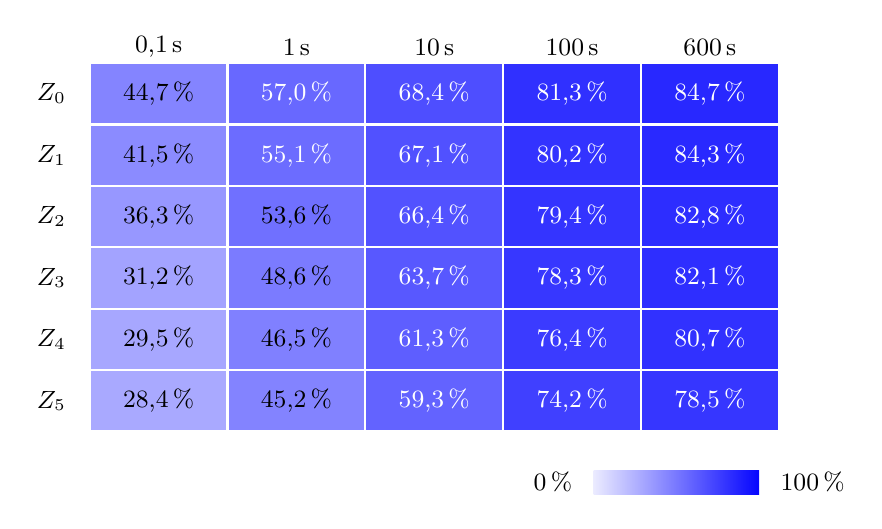
\begin{tikzpicture}[font=\small]
    \def\cellw{1.75}
    \def\cellh{0.78}

    \foreach [count=\col from 0] \label in {0{,}1\,s,1\,s,10\,s,100\,s,600\,s} {
        \node at ({\col*\cellw+0.5*\cellw},{6*\cellh+0.20}) {\label};
    }

    \newcommand{\drawlevelrow}[3]{%
        \node[anchor=east] at (-0.18,{#1*\cellh+0.5*\cellh}) {#2};
        \foreach [count=\col from 0] \value in {#3} {
            \pgfmathsetmacro{\mix}{8+0.9*\value}
            \pgfmathtruncatemacro{\dark}{\value>55}
            \ifnum\dark=1\def\textcolor{white}\else\def\textcolor{black}\fi
            \fill[blue!\mix!white]
                ({\col*\cellw},{#1*\cellh})
                rectangle ++(\cellw,\cellh);
            \draw[white,line width=0.8pt]
                ({\col*\cellw},{#1*\cellh})
                rectangle ++(\cellw,\cellh);
            \node[text=\textcolor]
                at ({\col*\cellw+0.5*\cellw},{#1*\cellh+0.5*\cellh})
                {\pgfmathprintnumber[
                    fixed,fixed zerofill,precision=1,use comma
                ]{\value}\,\%};
        }
    }
    \drawlevelrow{0}{$Z_5$}{28.4,45.2,59.3,74.2,78.5}
    \drawlevelrow{1}{$Z_4$}{29.5,46.5,61.3,76.4,80.7}
    \drawlevelrow{2}{$Z_3$}{31.2,48.6,63.7,78.3,82.1}
    \drawlevelrow{3}{$Z_2$}{36.3,53.6,66.4,79.4,82.8}
    \drawlevelrow{4}{$Z_1$}{41.5,55.1,67.1,80.2,84.3}
    \drawlevelrow{5}{$Z_0$}{44.7,57.0,68.4,81.3,84.7}

    \node[anchor=east] at ({5*\cellw-2.5},{-0.64}) {0\,\%};
    \shade[left color=blue!8!white,right color=blue!98!white]
        ({5*\cellw-2.35},{-0.80}) rectangle ({5*\cellw-0.25},{-0.50});
    \node[anchor=west] at ({5*\cellw-0.10},{-0.64}) {100\,\%};
\end{tikzpicture}
\end{document}
